\documentclass[final,leqno,onefignum,onetabnum]{siamltexmm}
\usepackage{amsmath}
\usepackage{color,graphicx} 

\title{Detecting Hand movements from EEG Signals\thanks{Kaggle Grasp and lift competition. 
\url{https://www.kaggle.com/c/grasp-and-lift-eeg-detection}}} 

\author{Anirudhan J Rajagopalan, Michele Cer\'u\thanks{New York University (\email{ajr619@nyu.edu}; \email{mc3784@nyu.edu}). Questions, comments, or corrections to this document may be directed to this email address.}}

\begin{document}
\maketitle

\begin{abstract}
  This project aims to detect and classify the grasp and lift hand movements of a subject from EEG (Electroencephalography) recordings.
  Successful identification and classification of the recordings will help in developing Brain Computer Interfaces (BCI) that can be used to restore the ability of patients to do day-to-day tasks.
  We are provided with \~24 series of grasp and lift actions performed by twelve subjects.  We run our models using the first \~18 series as our training and the last \~2 series as our test set.
  We use the level1 predictions of the Kaggle contest winners as our baseline and try to compare the performance of our model against the level1 predictions of baseline.
  Using our simple pipeline we are able to show that we can get accuracy of 0.61 Mean Area Under the Curve (MAUC)\@.
\end{abstract}

\section{Introduction}

Electroencephalography (EEG) is used to record electrical activity of the brain.
It is typically noninvasive, with the electrodes placed along the scalp.  
In the Grasp And Lift (GAL) experiment twelve subjects were asked to perform lifting series in which the object's weight (165, 330, or 660g), surface friction (sandpaper, suede, or silk surface), or both, were changed unpredictably between trials, thus enforcing changes in fingertip force coordination.\cite{naturegal}
The hand movement of the subject was recorded by 3D sensors which were synchronized with the EEG cap thus providing us with the exact moment at which the GAL events happen.  With respecct to our goal of classifying the hand movements, we have to detect the following six events.

\begin{enumerate} 
  \item \textit{HandStart}: Beginning of the movement.
  \item \textit{FirstDigitTouch}: Making contact with the object.  
  \item \textit{BothStartLoadPhase}: Starting to load the object. 
  \item \textit{LiftOff}: Holding the object up.
  \item \textit{Replace}: Replacing the object in its original position.
  \item \textit{BothReleased}: Releasing the fingers from the object. 
\end{enumerate}

The EEG signals recorded by 32 electrodes fixed to the scalp are recorded at a frequency of 500Hz.  An added objective of this task is to make sure that we dont use any future data for doing predictions (No future data rule, as described in the data page of the challenge).  This restriction is imposed to mimic the real life scenarios in which such an application can be used, wherein, we will not have access to any of the future data while making predictions in real life.\cite{website:kaggle-competition}


This project aims to classify the hand movements of subjects by using EEG signal data.  We compare the performance of LinearSVM and GaussianSVM combined with VLAD and Bag of Features (BOF) feature representations.  We base our performance using the Area Under the Curve as described in the Kaggle challenge.  We try to reason the performance of our model with respect to the dataset by analysing the spatial relationship and variance of the features.  We then discuss about models that we might use to tackle this hard problem.

\section{Dataset Description}

\subsection{Sources and Format}
The dataset is provided by Kaggle Inc.\ for their Grasp and Lift Detection challenge\cite{website:kaggle-competition} sponsored by Way Consoritum\cite{website:way_consoritum}.  
The dataset consists of separate test and train zip files of size 153 MB and 915 MB respectively.  
The dataset expands to 447 MB and 3.1GB after extraction.  
Out of these datafiles, we cannot use the testset as they are being used for the competition submissions.  
The testset has only the *\_data.csv files with no corresponding *\_events.csv file.  
Since there is no *\_events.csv file we will not be able to learn or evaluate the performance of our models by using the test dataset provided in the challenge website.
So our effective usable dataset is only the training data which we partition into train and test set for training our models.

The dataset consists of two types of files: 
\begin{enumerate}
  \item{data.csv} --- CSV of series labels and values from the 32 electrode signals.
  \item{event.csv} --- CSV of series labels and event values.
\end{enumerate}
The sample dataset is included below for reference.

\begin{figure}[ht!]
  \centering
  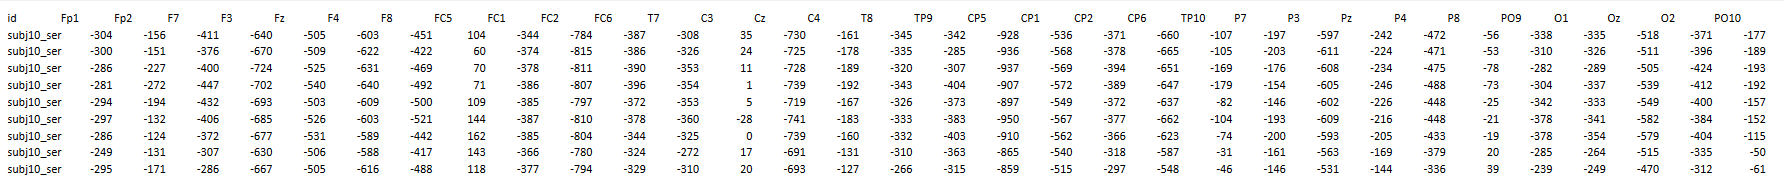
\includegraphics[width=1\textwidth]{images/sample_data}
  \caption{Sample Data format\label{fig:Sample_data}}
\end{figure}

\begin{figure}[ht!]
  \centering
  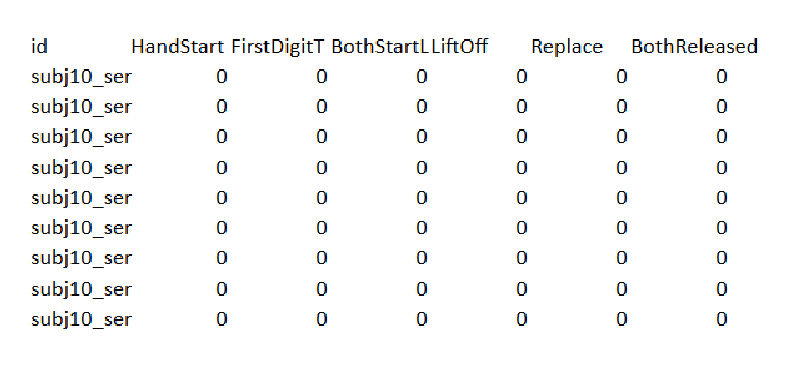
\includegraphics[width=0.5\textwidth]{images/sample_events}
  \caption{Sample Event format\label{fig:sample_events}}
\end{figure}

The event dataset will have a value of 1 corresponding to the event (stimulus) that is being performed at the instant of sampling.  There can be situations where there are multiple stimulus being triggered for the same EEG signal.  The objective is to classify (or) label the input EEG signals to the corresponding stimulus.

The total number of samples across the complete dataset is 17985850.

The spatial relationship between each of the 32 electrodes is given by Fig.~\ref{fig:eeg_spatial_relation}

\begin{figure}
  \centering
  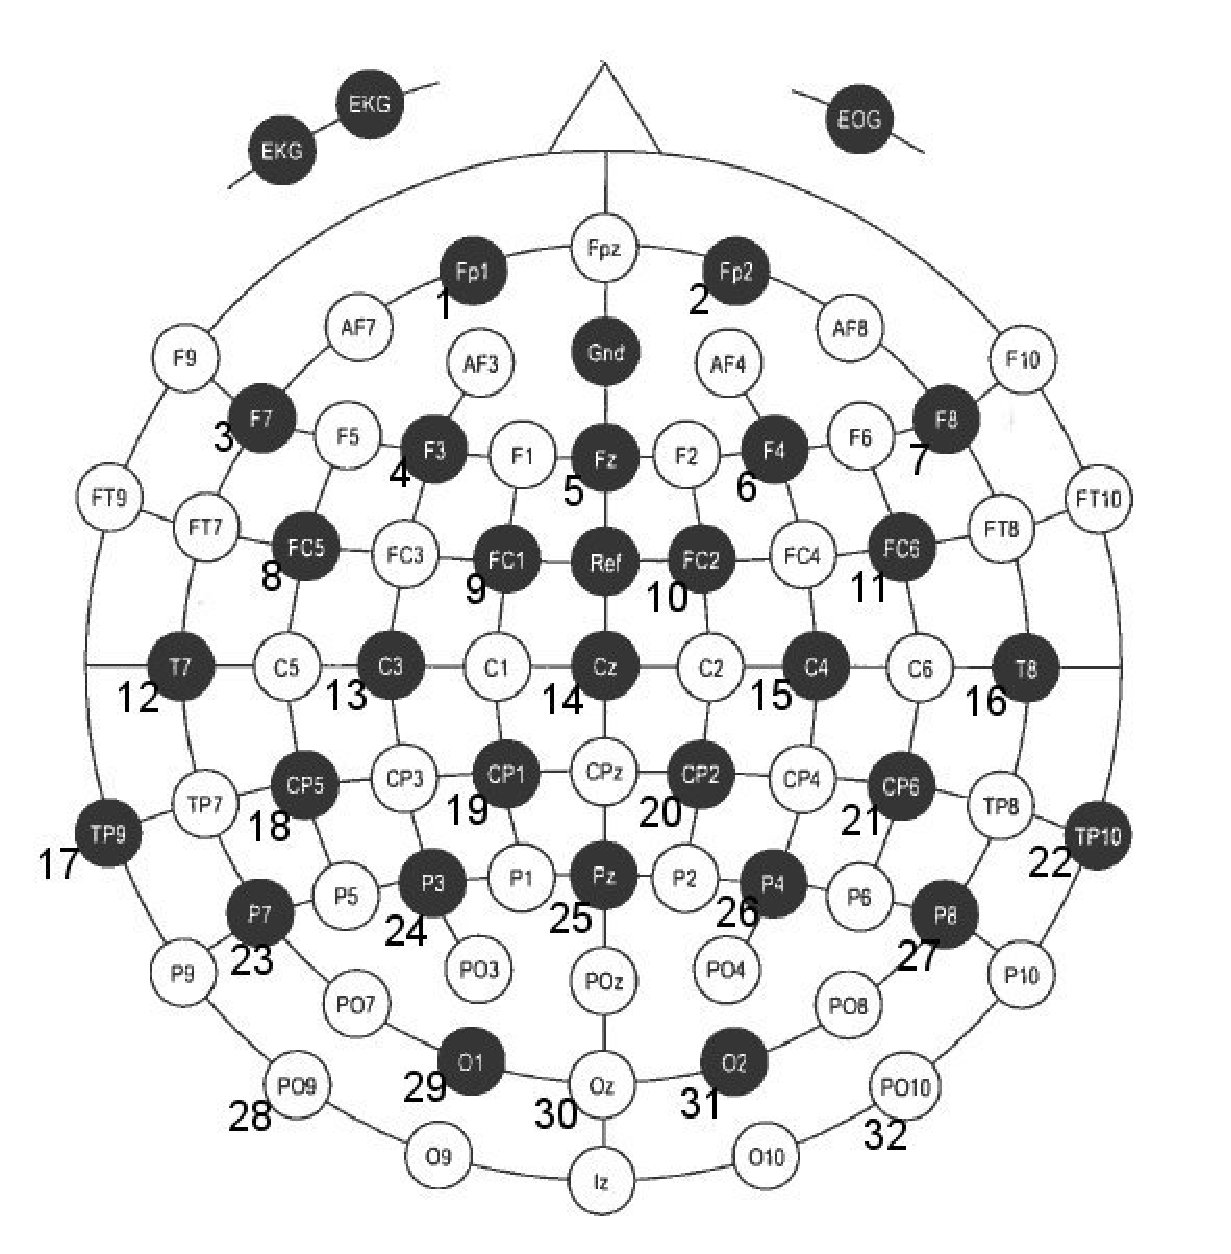
\includegraphics[width=0.5\textwidth]{images/eeg_spatial}
  \caption{Spatial relationship between 32 electrodes.\label{fig:eeg_spatial_relation}} 
\end{figure}

\subsection{Multilabeling or Multiclass classification}
The dataset can have multiple stimulus at the same time as shown in figure~\ref{fig:label_or_class}.
This is an important feature to consider as it forms the distinction between multiclass and multilabel classification problem.
\begin{figure}[ht!]
  \centering
  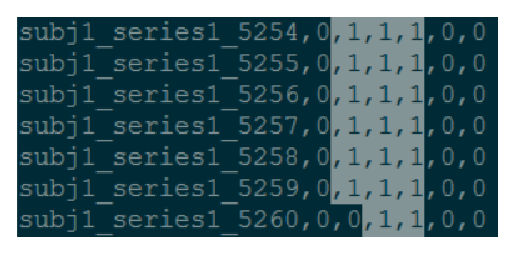
\includegraphics[width=0.5\textwidth]{images/multilabels}
  \caption{Multilabel or Multiclass classification problem.\label{fig:label_or_class}}
\end{figure}

\section{Problem Statement}
As described in the previous section, the objective is to classify/label the input EEG signals with their correspoinding stimulus.  
This is an inherently multilabel classification problem.  
We can reduce this to multiclass classification problem by considering the fact that the events happen in sequence.  
For example, BothReleased event is always followed by Replace which is always followed by LiftOff and so on and so forth.
Thus the problem of finding all events corresponding to the EEG signal can be decomposed into the problem of finding the start of the occurance of a particular event.

The constraint defined above simplifies our problem into a multiclass classification problem.  With proper feature selection and model selection we should be able to solve the problem effectively.

\section{Baseline}
\subsection{Choosing a baseline}
We considered the models developed by Alexandre Barachant (a.k.a cat) and Rafal Cycon (a.k.a dog) for our baseline model (Cat \& Dot solution)\cite{website:cat_dog_solution}.  
The solution by Cat and Dog won the first prize in the challenge and it makes logical sense to use that as our baseline.   
The cat and dog solution has three levels of models.


The first level of models uses 

\begin{enumerate}
  \item Covariance Matrices
  \item Event Related Potentials (ERP)
  \item Filter Banks
\end{enumerate}

The solution uses an ensemble of multiple learning models such as Logistic Regression with LDA, Convolutional Neural Network, and Recurrent Neural Networks.  
This model fits our requirement to be a baseline and hence we choose the Level-1 model of \textit{Cat and dog solution} as our baseline models.
We decided to compare the performance of the baselilne with respect to our own model.
The accuracy achieved by the Level-1 models are not readily available.  So we tried to run the baseline to get the accuracy values.

\subsection{Running the baseline}
The hardware specs listed in the \textit{Cat and Dog solution} page details the hardware used and the time taken for the entire pipeline.  
Considering that we are using only the Level-1 models as our baseline, we decided to try running the baseline to get a accurate idea of time and performance for Level-1 alone.

\subsubsection{Attempt 1}
We first attempted to run the Level-1 models in our own machines just to get an idea of how much memory and time requirements the Level-1 took.
We started out by installing all the packages specified in the requirements document and then started with the preprocessing step.
The preprocessing step ran successfully even in our local machine and created two numpy binary files \textit{infos\_val.npy} and \textit{infos\_test.npy}.
The numpy files are to be consumed by the baseline files for building the models.


We ran the baseline using \textit{lvl1/genAll.sh} in our local.  The baseline crashed due to out of memory.  Thus we decided to run all our experiments in New York University (NYU)'s High Performance Computing (HPC) clusters\cite{website:nyuhpc}.


\subsubsection{Attempt 2}
The second attempt\cite{website:attempt_2} involved trying to run the Level-1 code using NYU HPC clusters.
\begin{enumerate}
  \item As used in the first attempt, we decided to treat the baseline as a blackbox and try to run the baseline code.
  \item We identified out the entry point for the baseline models and decided to run the model in NYU HPC clusters.
  \item We figured out the modules required to make all the python packages used in the baseline to work and loaded the modules.
  \item We submitted a HPC job for running the baseline.  The job requested for the exact number of CPU nodes, CPU cores, GPU resource and RAM mentioned in the Hardware specs. 
\end{enumerate}

The second attempt to run the baseline also ended without success as the system crased due to mismatch between required packages and the available packages in HPC\@.

\subsubsection{Attempt 3}
Since running the baseline on HPC crashed and running the models on our local resulted in `out of memory' error, we decided to run the baseline in our local using a fraction of the sample.

\begin{enumerate}
  \item We started out by trimming the input files from 18 series of GAL to just 6 series of GAL per subject.
  \item This corresponds to just \~4000 lines of samples per input file and we were able to load the data in our local effectively.
  \item We installed the exact version (including the minor versions) of almost all the packages specified in the baseline.
  \item A few packages that were mentioned in the baseline were not available due to some mysterious reason and we had to install the previous version for these packages.
  \item We ran the baseline with the subsample of the original dataset.
\end{enumerate}

We still ran into a number of issues while running the code.  Our guess is that the code in the \textit{Cat and Dog Solution}'s repository has got some breaking changes after the final submission.  We emailed the authors regarding the issue and even after help from the authors we were unable to get the baseline running.

\subsection{Baseline Results}
As discussed above, since we couldn't get the baseline running even after 3 attempts and the help of the authors and since we had spent more than 2 weeks on this problem, we decided to move ahead with building our own solution to this interesting problem.


The attempt to run the baseline gave us significant insights into the Domain, data and assumptions that can be used for solving the problem.

\section{Building our own Pipeline}

\subsection{Understanding the domain}
The biggest challenge for building the pipeline was to understand the domain and figure out the preprocessing tasks.  
The components downstream the pipeline was already fixed to be VLAD\cite{art:vlad_aggregate_paper}\cite{art:all_about_vlad}  and Bag of Features.
After a bit of exploring and a bit of guidance from our professor we decided to use MNE\cite{website:mne_python} for the data preprocessing.  MNE provided us with a number of tools for preprocessing the data.
\begin{enumerate}
  \item Epochs
  \item Covariance measures
  \item XDawn filter\cite{art:Xdawn_filter}
  \item Algorithms to process the raw data and generate the Event Related Potentials.
\end{enumerate}
We made good and extensive use of the codebase of \textit{Cat and Dog} solution to understand the type of preprocessing that was carried out by them.  
We also went through the forum of the Kaggle challenge to gather insight about the domain and ways of processing the data.


\subsection{Data Preprocessing}

We used MNE to consume the raw data in csv format to find the epoch values and the Event Related Potentials.  
We also use MNE to get the covariance matrix on the complete training/test dataset.  
This information is then fed to xDawn filter with WINDOW size as 500.  
The value of the parameter num\_components for xDawn, which determines the number of features in the processed data was varied from 2 to 4 and the resulting three dimensional array was saved in numpy binary formats.

The total run time for data preprocessing took around an hour for the dataset.

\subsection{Exploring the preprocessed data}
We then set out to explore the processed data to better understand the dataset.
\subsubsection{Clustering of local descriptors}
The total number of stimulus that has to be classified is six.  
Any classification task becomes easier if we find that the data is separable by some degree.  
Since our model essentially depends on builing over the clusters formed by local descriptors, we decided to cluster the data to find if there is any amount of separatbility of data.

We ran experiments to cluster the local descriptors for one subject (Subject 1 in the dataset) using MiniBatchKMeans algorithm.  
We then used the cluster information and different markers to plot the cluster information on a two dimensional plot by reducing the dimensionality.
The plot generated for n\_components = 2 is shown as an example in Fig~\ref{fig:local_descriptors_clusters}.

\begin{figure}
  \centering
  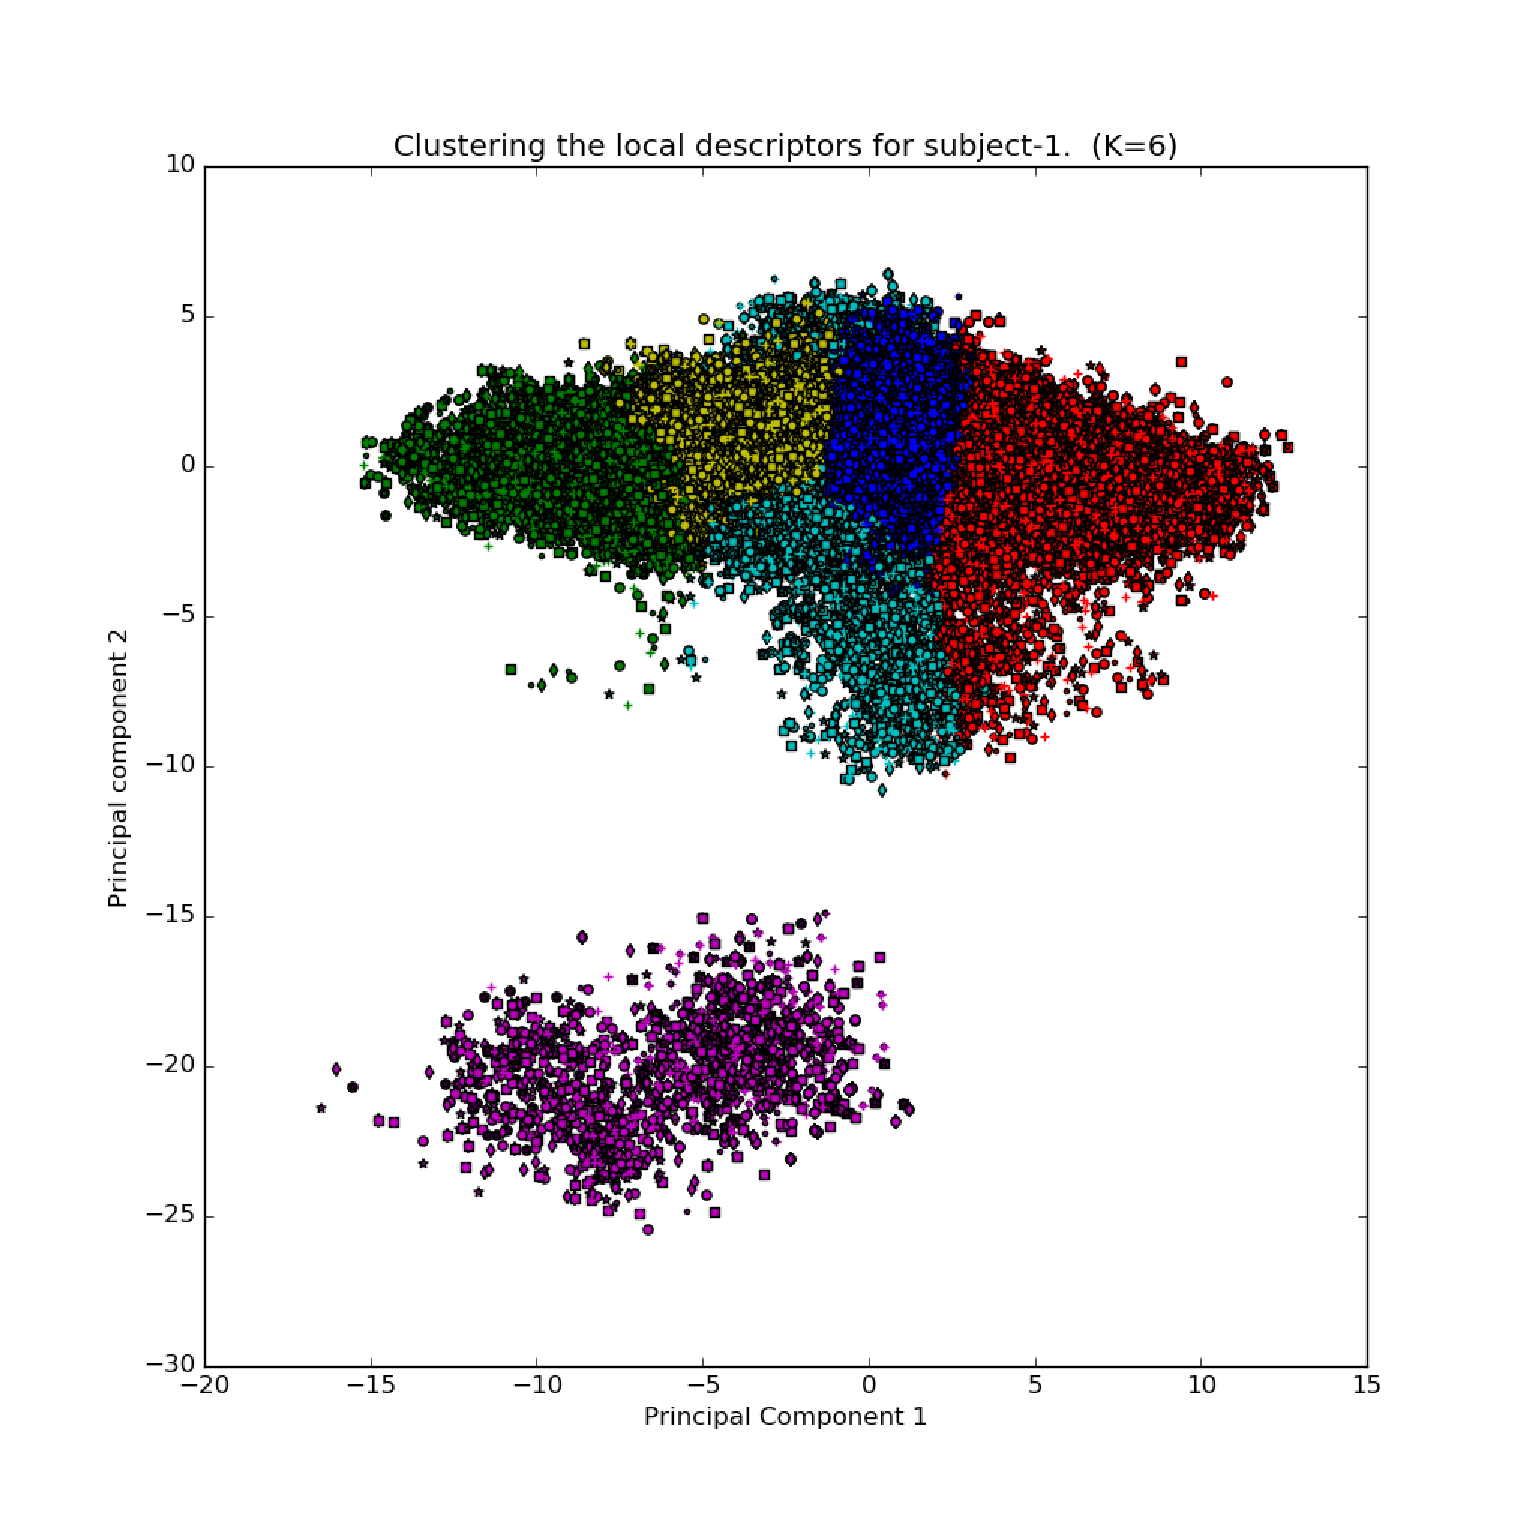
\includegraphics[width=0.75\textwidth]{images/cluster_centers}
  \caption{Clustering the local descriptors of a single subject into 6 clusters.  Different clusters are represented by different colors.  The local descriptors that gives raise to a particular stimulus are denoted by different markers such as plus, star, circle, square and so on.  Just a cursory look on the clusters makes it clear that there data is not separable easily.\label{fig:local_descriptors_clusters}} 
\end{figure}

\subsubsection{Variance of local descripitors}
PCA is a technique for dimensionality reduction.  
It works by finding components that provide the maximum variance (It can be thought of as the direciton in which the features spread out the most).
Finding the variance of the features helps us to understand how the data is spread and how much dimensions we should use to tackle the learning problem.  
We created a plot of the variance of a the local descriptors for a subsample of the dataset (Subject 1).  
The variance curve is as shown in Fig~\ref{fig:ld_variance}

\begin{figure}
  \centering
  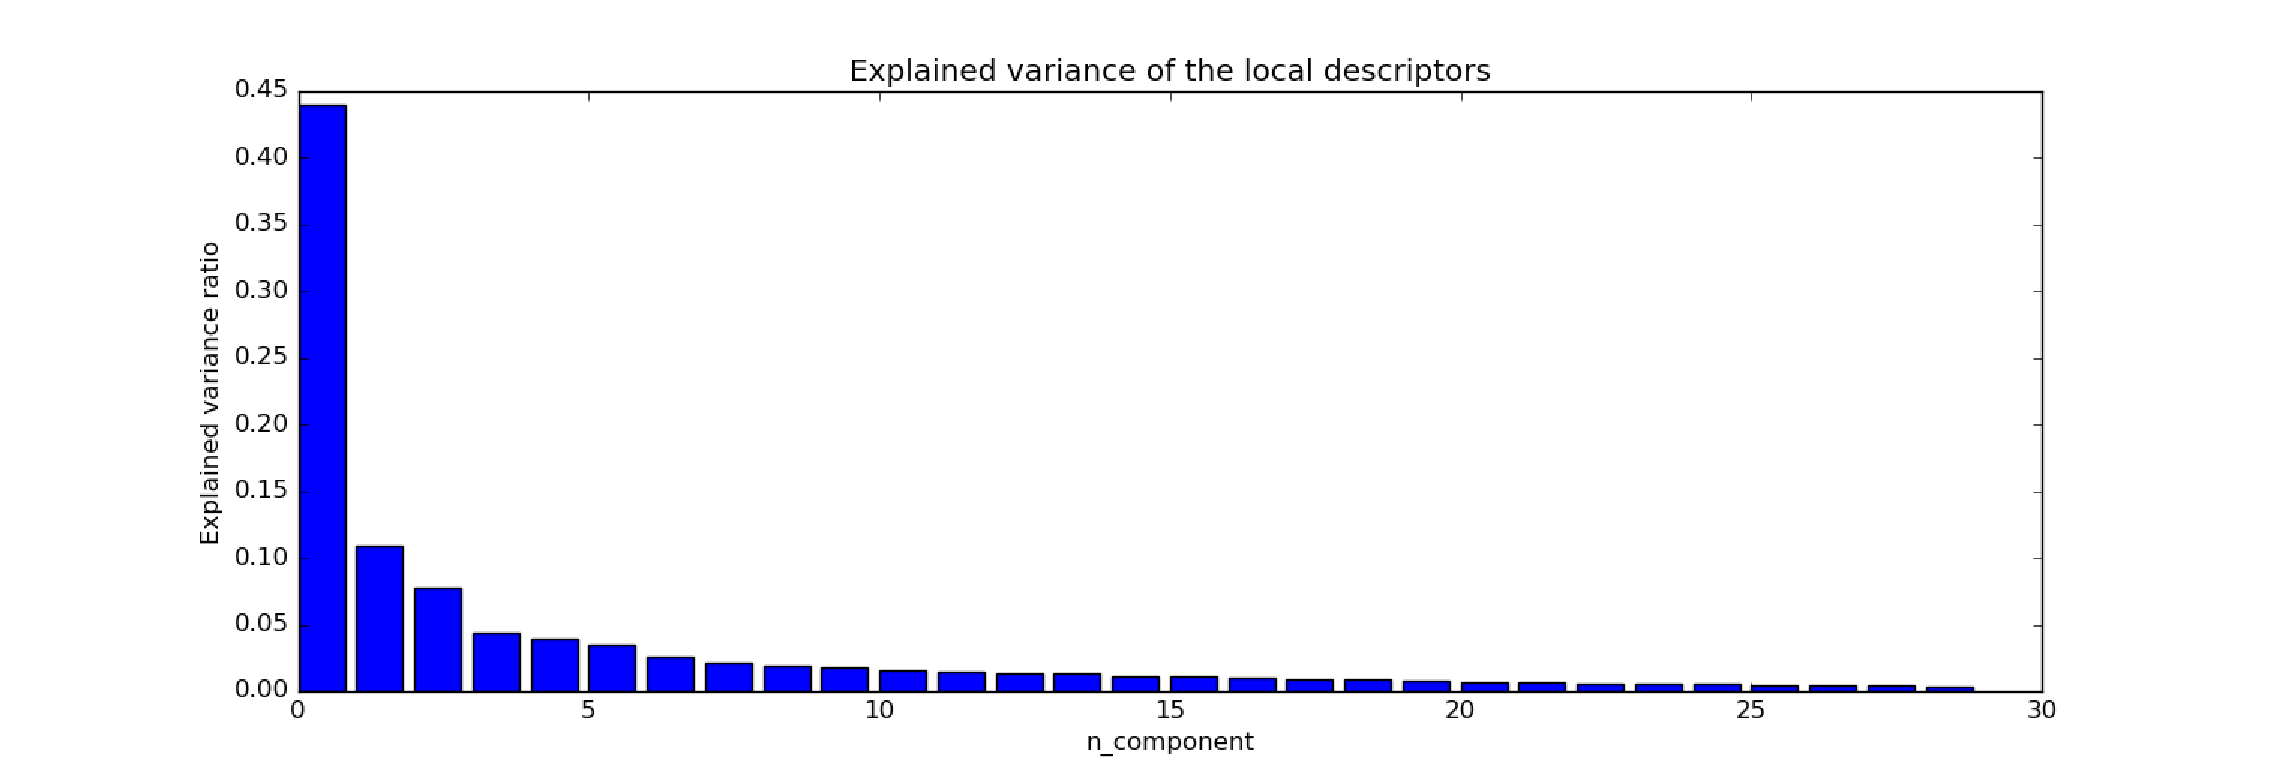
\includegraphics[width=0.75\textwidth]{images/ld_variance}
  \caption{Explained variance ratio of local descriptors for a subsample (Subject 1).  We get variance measures of 99, 95, 90, 77, 65 and 50 for components 29, 21, 16, 7, 4, 2 respectively.\label{fig:ld_variance}} 
\end{figure}

The analysis of variance was actually performed after we got the results for BOF and Vlad models.  This makes us wonder whether the model's performance might have increased if we had used PCA on the local descriptors before applying our models.

\newpage

\bibliographystyle{siam}
\bibliography{references}

\end{document}
